%\documentclass[aps,prb,twocolumn,showpacs]{beamer}
\documentclass[]{beamer}
%\usetheme{Berkeley}

\usepackage{graphicx}
\usepackage{amsfonts}
\usepackage{amssymb}
\usepackage{amsmath}
\usepackage{mathrsfs}
\usepackage{braket}
\usepackage{epstopdf}
%\usepackage{geometry}
\usepackage{wrapfig}
%\geometry{margin=1in}

\def\avg#1{\langle#1\rangle}
\def\v#1{\mathbf{#1}}
\def\Re {\mbox{Re}}
\def\Im {\mbox{Im}}
\def\tr{\mbox{tr}}
\def\nn{\nonumber}
\def\pp{\parallel}
\def\ket#1{\vert #1 \rangle}
\def\bra#1{\langle #1 \vert}
\def\me#1#2#3{\langle #1 \vert #2 \vert #3 \rangle}
\def\Br{\mathbf{r}}

\newcommand{\kp}{k_{+}}
\newcommand{\ki}{k_{-}}
\newcommand{\idz}{i\partial_z}
\newcommand{\kperp}{\mathbf{k}_\parallel}

\title{Thesis Proposal: \\Nanostructures with Topological Insulators}
\author{Mahmoud Lababidi}



\begin{document}

%%%%%%%%%%%%%%%%%
\begin{frame}{}
\maketitle
\begin{figure}
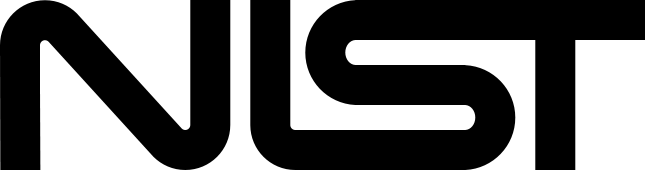
\includegraphics[width=1in]{include/nist.png}\quad

\includegraphics[width=1in]{include/gmu.eps}\quad

\includegraphics[width=1in]{include/onr.jpg}
\end{figure}
\end{frame}
%%%%%%%%%%%%%%%%%

\begin{frame}{Introduction}
Introduction to Topological Insulators\\
Spin-flip scatter on the surface of TIs\\
Superconducting proximity effect on TIs\\
Josephon junction structures on the surface of TIs\\
MOSFETs using TIs\\

\end{frame}
%%%%%%%%%%%%%%%%%

\begin{frame}{Introduction}
\maketitle
\end{frame}
%%%%%%%%%%%%%%%%%



\begin{frame}{Introduction}
\begin{figure}
\center
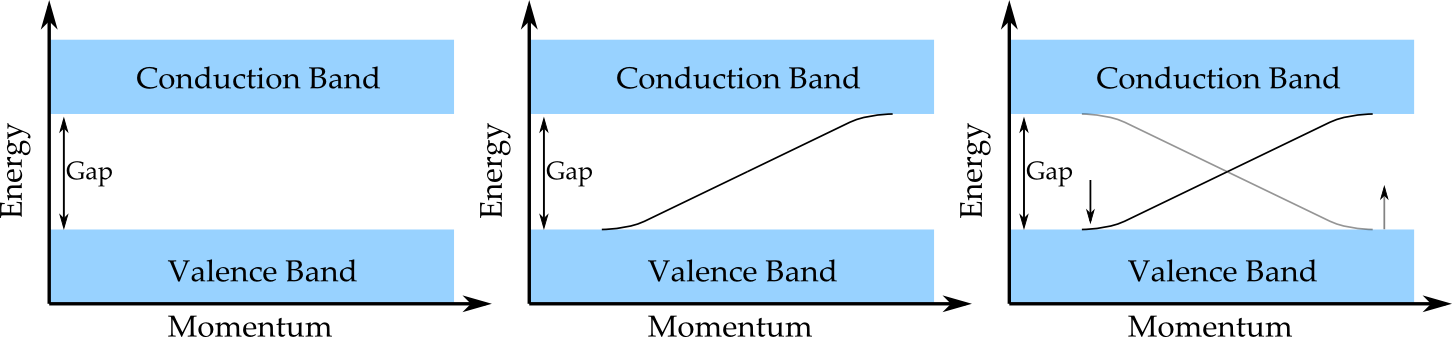
\includegraphics[width=4in]{bands2.png}

\end{figure}

(a) Energy spectrum of a trivial band insulator \\
(b)  Energy spectrum of a quantum hall state \\
(c)  Energy spectrum of a topological insulator \\

\end{frame}
%%%%%%%%%%%%%%%%%


\begin{frame}{Introduction}


\begin{figure}
\center
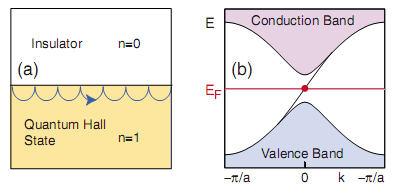
\includegraphics[width=3in]{qhall.png}

\end{figure}

\end{frame}
%%%%%%%%%%%%%%%%%

\begin{frame}{Introduction}
\begin{figure}
\center
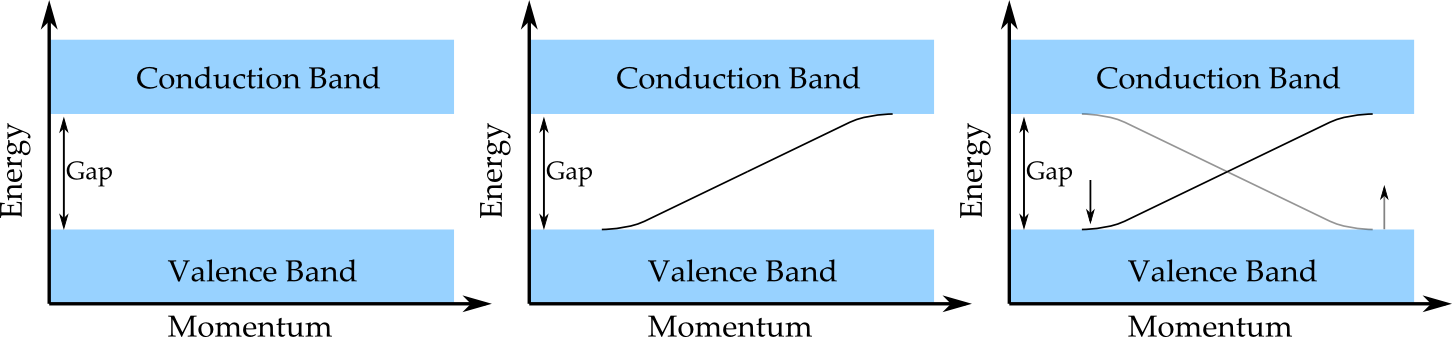
\includegraphics[width=4in]{bands2.png}

\end{figure}

(a) Energy spectrum of a trivial band insulator \\
(b)  Energy spectrum of a quantum hall state \\
(c)  Energy spectrum of a topological insulator \\

\end{frame}
%%%%%%%%%%%%%%%%%



\begin{frame}{Introduction}
$E = \pm(k^2 - M)$
\begin{figure}
\center
\includegraphics[width=4in]{bulk1}

\end{figure}
\end{frame}  


\begin{frame}{Introduction}
$E = \pm\sqrt{(k^2 - M)^2}$
\begin{figure}
\center
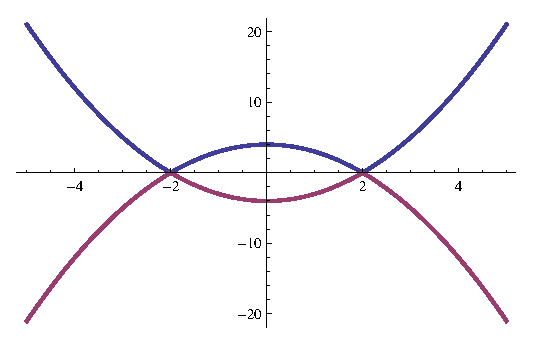
\includegraphics[width=4in]{bulk2}

\end{figure}
\end{frame}  


\begin{frame}{Introduction}
$E = \pm\sqrt{(k^2 - M)^2 +\alpha k^2}$ (spin-orbit)
\begin{figure}
\center
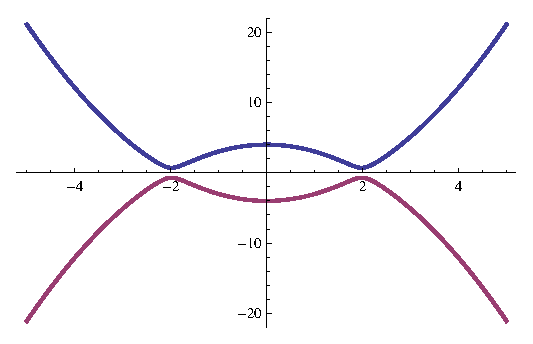
\includegraphics[width=4in]{bulk3}

\end{figure}
\end{frame}  
%%%%%%%%%%%%%%%%%%%%

\begin{frame}{Introduction}
\center
How do we get the connecting state between the valence band to the conduction band?\\
\end{frame}  
%%%%%%%%%%%%%%%%%%

\begin{frame}{Introduction}
\center
Let's try adding a boundary!
\end{frame}  
%%%%%%%%%%%%%%%%%%%%%%

\begin{frame}{Introduction}
\begin{figure}
\center
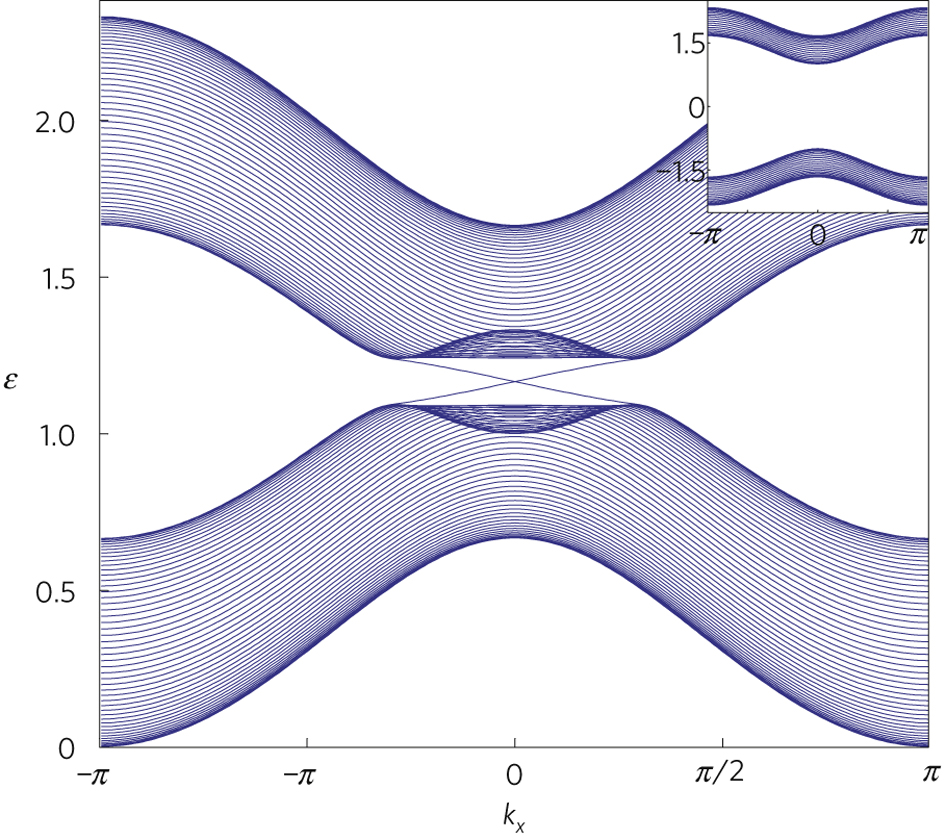
\includegraphics[width=4in]{floquet.jpg}

\end{figure}
\end{frame} 


\begin{frame}{Introduction}
\begin{figure}
\center
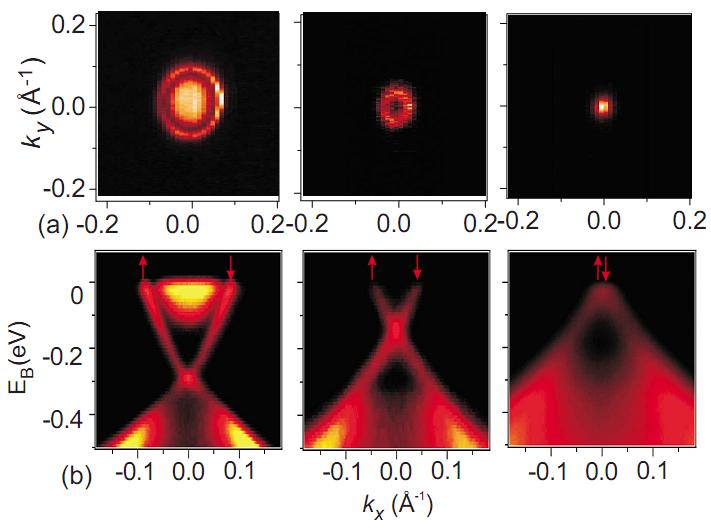
\includegraphics[width=4in]{diraccone.png}

\end{figure}
\end{frame}  


\begin{frame}{Motivation and Background}
Insulating bulk with metallic surface states.\\
Surface Dirac Fermions which behave relativistically and zero mass\\
Dispersion: $E=\pm\hbar v k$ \\

Surface Hamiltonian
\begin{equation*}
H=\vec{\sigma}\cdot \vec{k}-\mu=\sigma_x k_x + \sigma_y k_y - \mu
\end{equation*}
$\sigma$ are the Pauli spin matrices, $\mu$ is the chemical potential.
\end{frame}
%%%%%%%%%%%%%%%%%

\begin{frame}{Applications}

Electronics \& Spintronics\\
Majorana Particles\\
$\rightarrow$Topological Quantum Computation\\
Topological order\\
Klein Tunneling\\
\end{frame}
%%%%%%%%%%%%%%%%%


\begin{frame}{Metal to TI Scattering}
\Large What is the physics of an electron scattering off of a TI surface?
\end{frame}
%%%%%%%%%%%%%%%%%


\begin{frame}{Metal to TI Scattering :}
\begin{figure}
\center
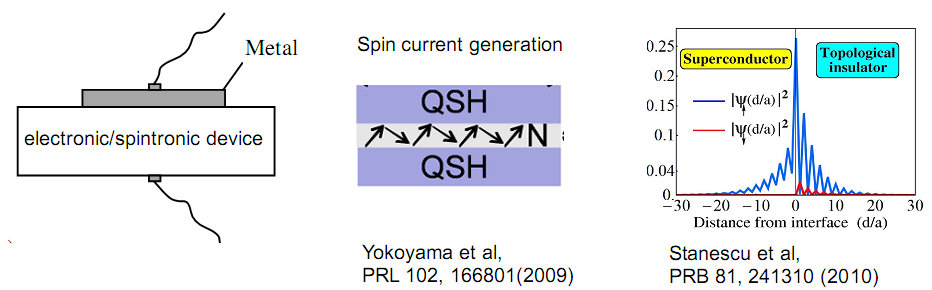
\includegraphics[width=3.4in]{devices.png}
\end{figure}
\end{frame}
%%%%%%%%%%%%%%%%%


\begin{frame}{Metal to TI Scattering}
\begin{figure}
\center
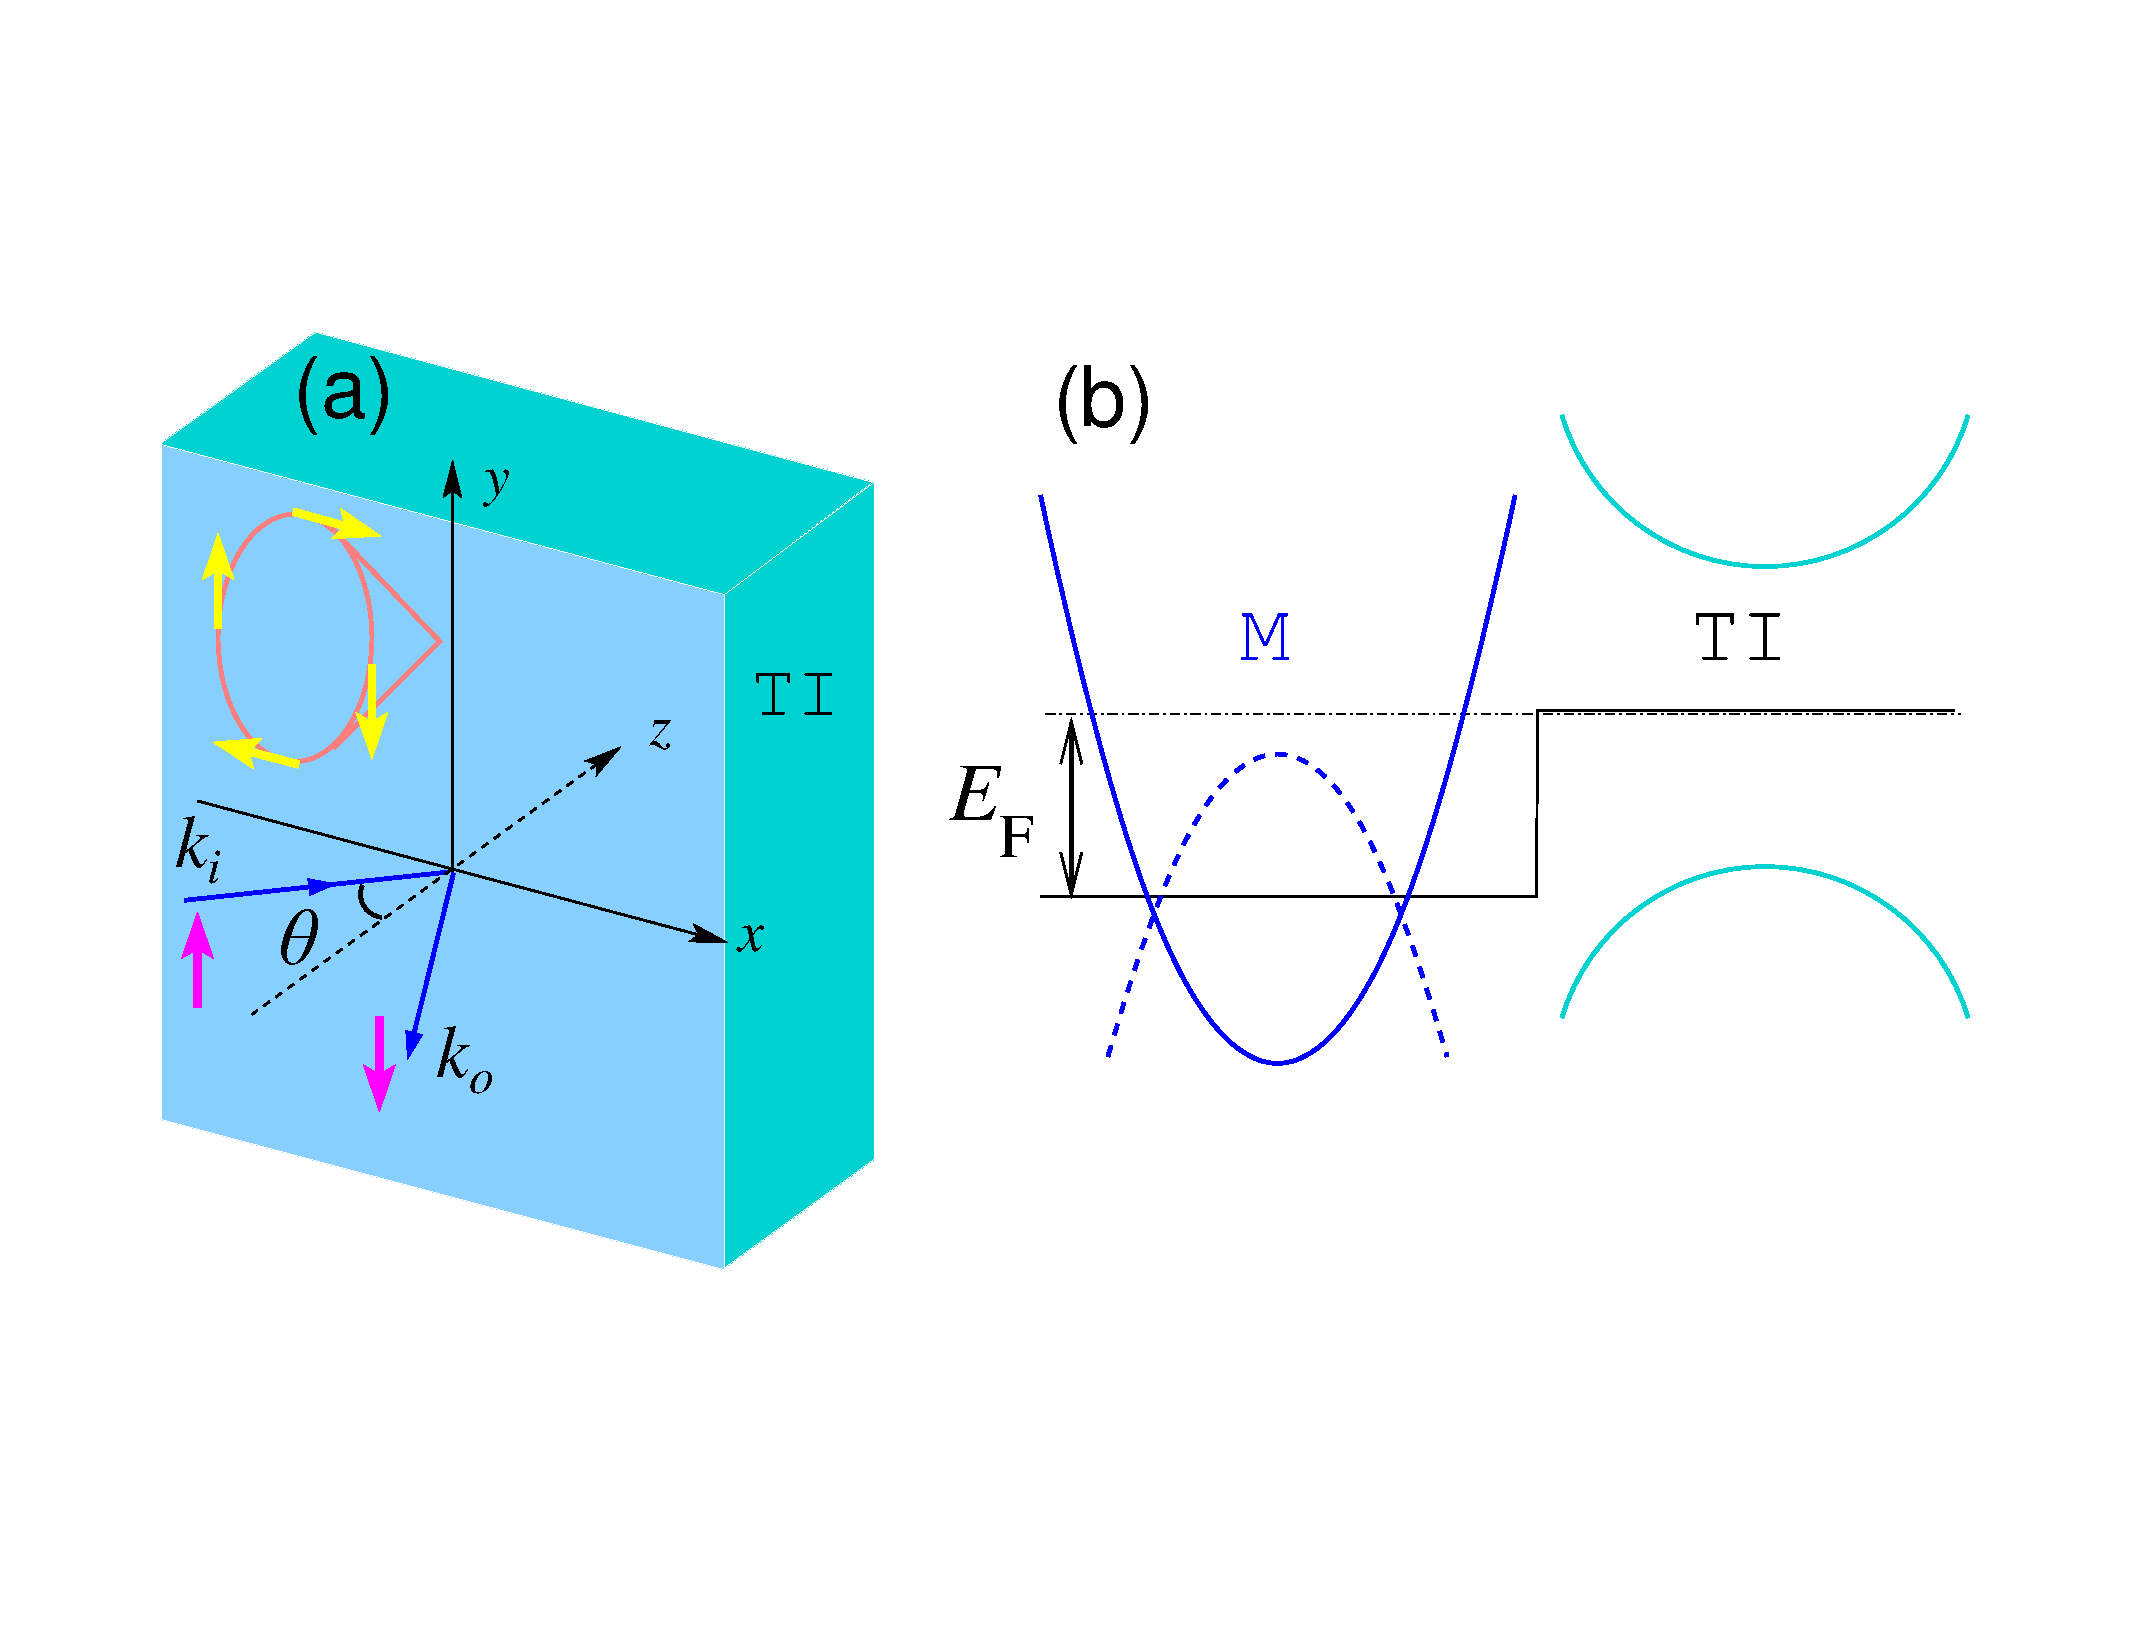
\includegraphics[width=3.4in]{geometry.pdf}
\end{figure}
(a) Scattering geometry at a metal (M)-topological insulator (TI) interface.\\
(b) Schematic band structure of the metal (modeled by $\hat{H}_M$) and topological insulator.
\end{frame}
%%%%%%%%%%%%%%%%%





\begin{frame}{Metal to TI Scattering}

%The scattering matrix has the general form \cite{mott}
%\[
%\hat{S}_{Mott}=u\hat{1}+w\hat{{\boldsymbol{\sigma}}}\cdot (\mathbf{k}_{i}\times %\mathbf{k}_{o}),
%\]

The scattering (reflection) matrix has the form
\[
\hat{S}(\v{k})=\left(
\begin{array}{ll}
  g & \bar{f}   \\
  f & \bar{g}
  \end{array}
\right),
\]
where $|g|^2+|f|^2=1$ and  $\alpha=\mathrm{Arg}(g^*f)$

The wave function inside the metal ($z<0$):
\[
\hat{\Phi}_M=(r_1e^{-ik'_{z} z},r_2e^{-ik'_{z}z},e^{ik_{z}z}+g e^{-ik_{z}z} ,f e^{-ik_{z}z})^{\mathrm{T}},
\]

Ben-Daniel and Duke boundary condition:
\[
\hat{\Phi}_M=\hat{\Phi}_{TI}, \;\;\; \hat{v}_M \hat{\Phi}_M = \hat{v}_{TI}\hat{\Phi}_{TI}.
\]

velocity matrix $\hat{v}_{i}=\partial \hat{H}_i/\partial k_z$, $i\in \{M, TI\}$. 


\end{frame}
%%%%%%%%%%%%%%%%%




\begin{frame}{Metal to TI Scattering}
\begin{wrapfigure}{r}{.5\textwidth}
\vspace{-50pt}
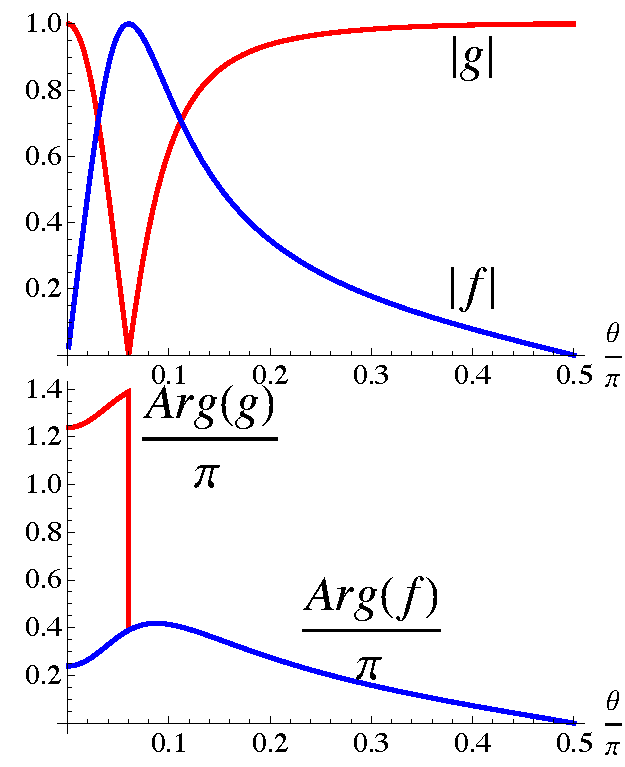
\includegraphics[width=2.4in]{scatt.pdf}
\end{wrapfigure}
The magnitudes (upper panel) and \\ 
the phases (lower panel) of the \\
spin-flip amplitude $f$ and \\
spin-conserving amplitude $g$ \\
versus the incident angle $\theta$. \\
$E=0.1$eV, $E_F$=0.28eV. $|g|^2+|f|^2=1$.

\end{frame} 




\begin{frame}{Metal to TI Scattering: Spectral Function}

%%%%%%%%%%%%%%%%%%%%%%%%%%
\begin{figure}
\center
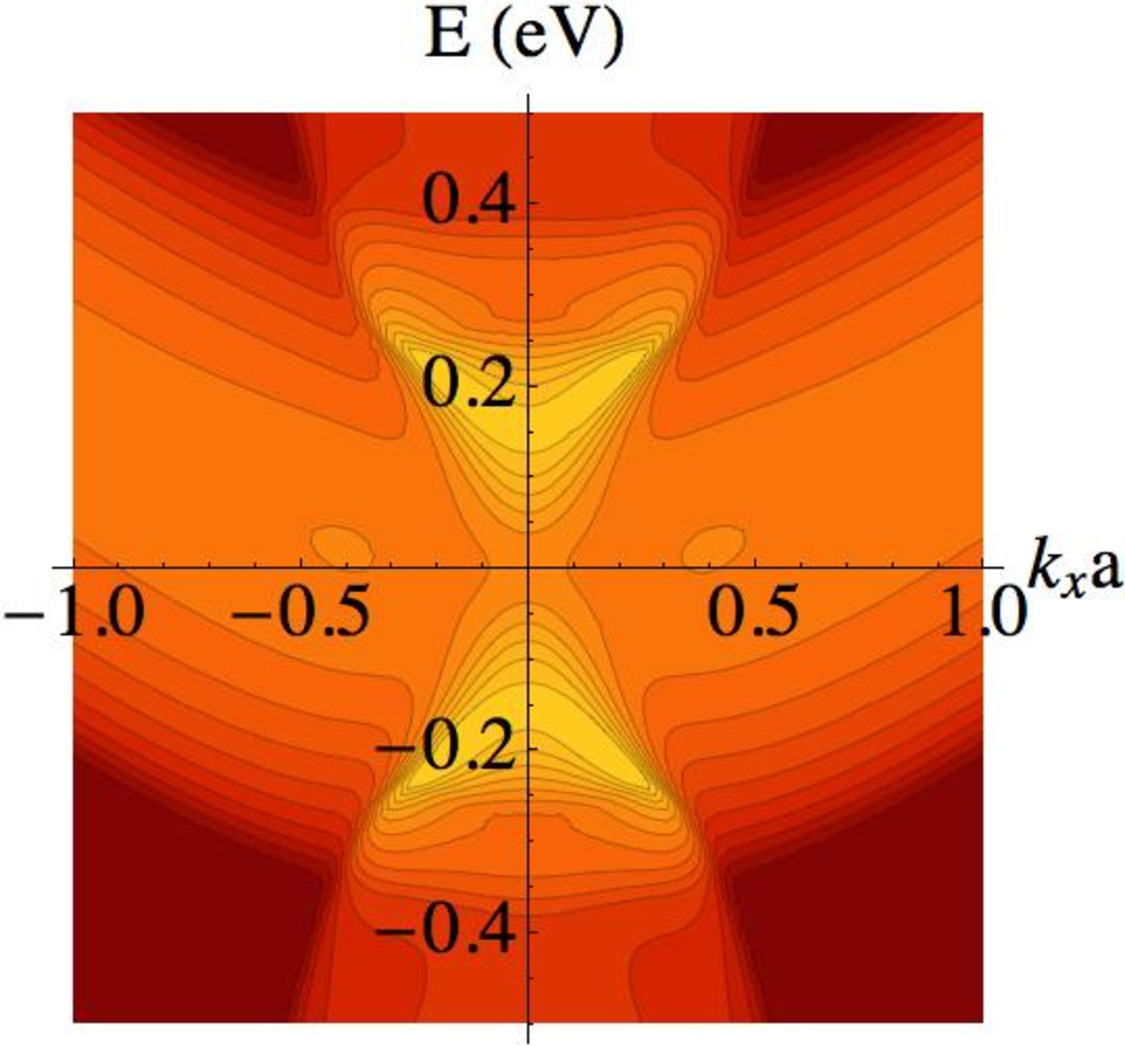
\includegraphics[width=1.7in]{j1.pdf}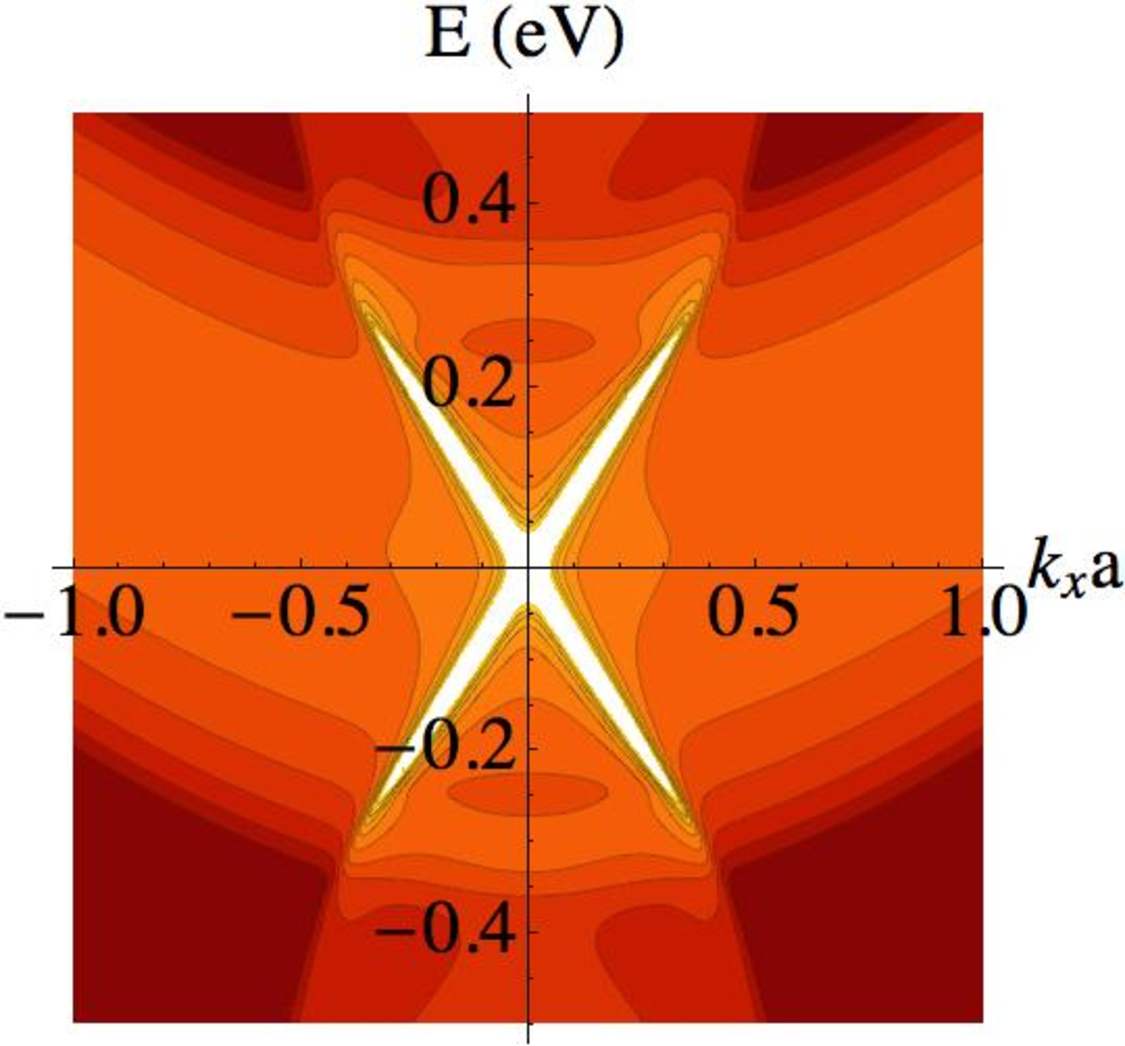
\includegraphics[width=1.7in]{j2.pdf}
\end{figure}
The spectral function $N(E,k_x,k_y=0)$ at the interface of M-TI\\
Left:  good contact, $J=t_M$, showing the continuum of MIGS. \\
Right: poor contact, $J=0.2t_M$ showing Dirac spectrum\\
$t_M=0.18eV$, $\mu_M=-4t_M$, $a$ is lattice spacing.
%%%%%%%%%%%%%%%%%%%%%%%%%%
 
\end{frame}
%%%%%%%%%%%%%%%%%




\begin{frame}{Metal to TI Scattering}

%%%%%%%%%%%%%%%%%%%%%%%%%%
\begin{figure}
\center
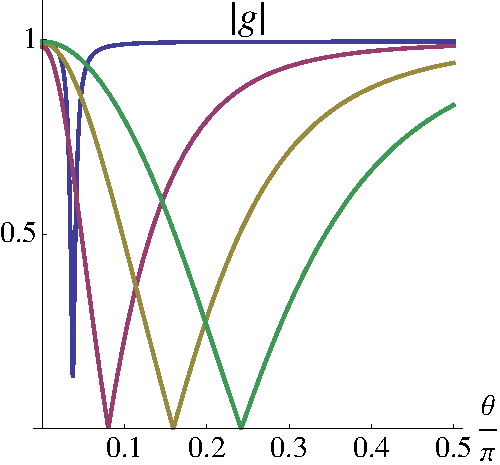
\includegraphics[width=1.7in]{la1.pdf}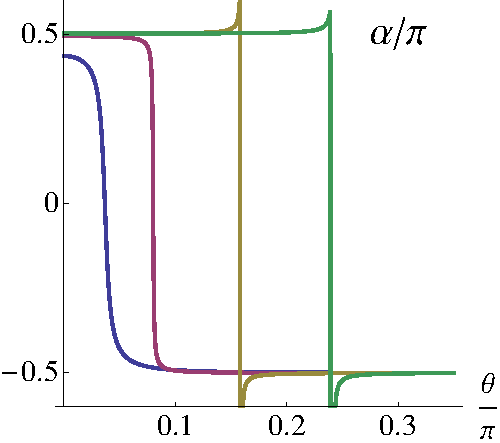
\includegraphics[width=1.7in]{la2.pdf}
\end{figure}
%%%%%%%%%%%%%%%%%%%%%%%%%%
%The spin-conserving reflection amplitude $|g|$ and spin rotation angle 
%\alpha$ versus the incident angle $\theta$ for increasing contact transparency,

$J/t_M=0.25, 1, 1.5, 2$ (from left to right). $t_M=0.18eV$, $\mu_M=-4t_M$, $E=0.05$eV, $k_y=0$.
%$|f|^2=1-|g|^2$. 
\end{frame}
%%%%%%%%%%%%%%%%%




%%%%%%%%%%%%%%%%%%%%%%%
\begin{frame}{Metal to TI Scattering: Summary}
\begin{list}{*}{}
\item Critical incident angle at which complete (100\%) spin flip reflection\\ 
\item Well-defined Dirac cone in the tunneling limit\\ 
\item Good contacts: metal induced gap states
\end{list}
\end{frame}
%%%%%%%%%%%%%%%%%



%%%%%%%%%%%%%%%%%%%%%%%
\begin{frame}{Next}
\begin{list}{*}{}
\Large \center
Onto the superconducting proximity effect...
\end{frame}
%%%%%%%%%%%%%%%%%





\begin{frame}{The Fu-Kane Proposal}
%%%%%%%%%%%%%%%%%%%%%%%%%%
\begin{figure}
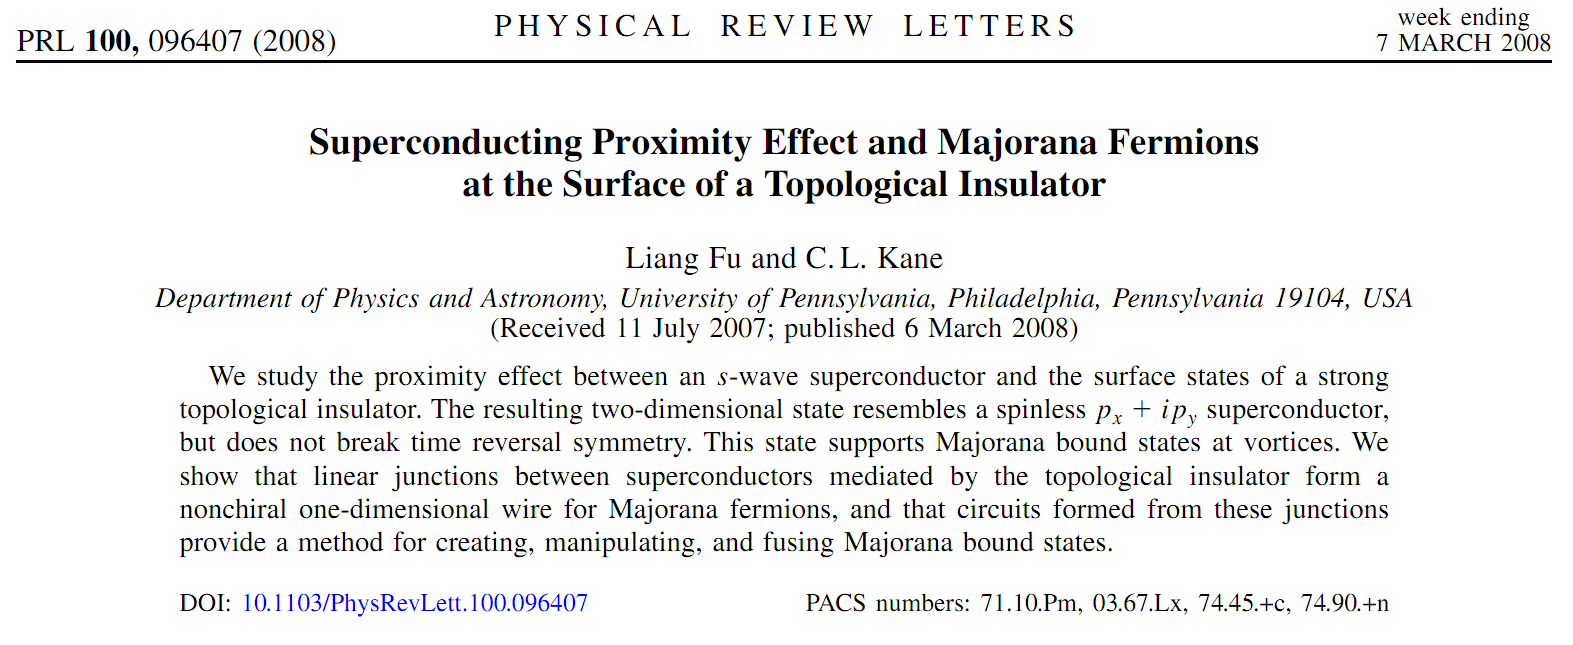
\includegraphics[width=4in]{include/fukane-prl.png}\\
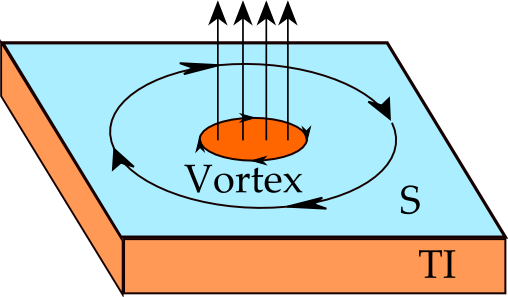
\includegraphics[width=2.5in]{include/majorana2.png}\\

\end{figure}
%%%%%%%%%%%%%%%%%%%%%%%%%%
\end{frame}


\begin{frame}{Majorana Modes: Topological Quantum Computing}
%%%%%%%%%%%%%%%%%%%%%%%%%%
\begin{figure}
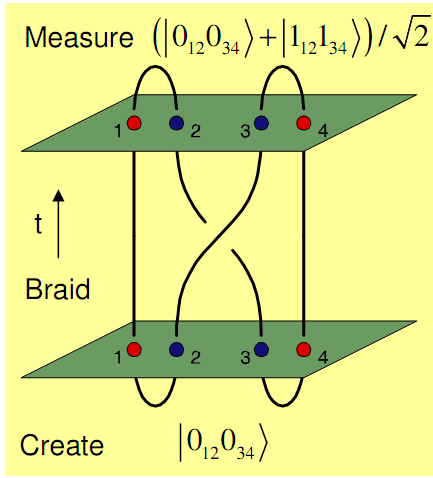
\includegraphics[width=2.5in]{include/braid.png}
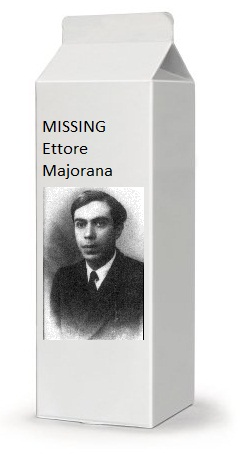
\includegraphics[width=1.5in]{include/milk-carton.jpg}

\end{figure}
%%%%%%%%%%%%%%%%%%%%%%%%%%
C. Kane - Exotic States of Matter Talk - Jan 14-2010
\end{frame}

\begin{frame}{Fu-Kane Model (Phenomenological)}
TI Surface Hamiltonian
\begin{equation*}
h_s(\mathbf{k})=-\mu_s + v_s (\sigma_xk_y-\sigma_y k_x),
\end{equation*}
Superconducting TI Surface Hamiltonian
\begin{equation*}
H_{FK}(\mathbf{k})=\left(
\begin{array}{cc}
h_s(\mathbf{k})  &  i\sigma_y  \Delta_s \\
-i\sigma_y \Delta_s^*  &   -h_s^*(-\mathbf{k})
\end{array}\label{fkmodel}
\right),
\end{equation*}
\begin{equation*}
 \mathbf{k}=(k_x,k_y),
\end{equation*}
Energy Dispersion
\begin{equation*}
E(k)=\sqrt{|\Delta_s|^2+(v_sk \pm\mu_s)^2}.
\end{equation*}
 \\
L. Fu and C. L. Kane, Phys. Rev. Lett. 100, 096407 (2008)
\end{frame}


\begin{frame}{Goals}
\Large
1) Verify Fu-Kane Model from self-consistent microscopic calculation\\
2) Order Parameter suppression\\
3) Triplet Pairing Correlations (due to SO Coupling) \\
\end{frame}



\begin{frame}{Geometry} 
\begin{figure}
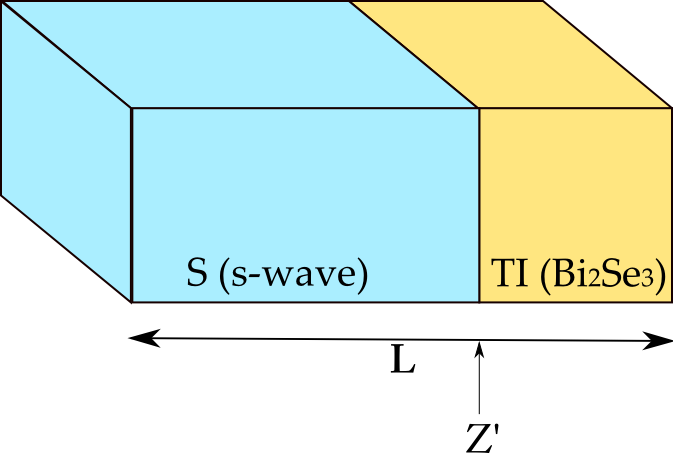
\includegraphics[width=3in]{include/block.png}\\
%Total Length: L, position of interface: z$^\prime$
\end{figure}
\end{frame}



%\begin{frame}{Cu$_x$Bi$_2$Se$_3$}
%%%%%%%%%%%%%%%%%%%%%%%%%%
%Model for Inspiration: 
%\begin{figure}
%
\includegraphics[width=4in]{include/hassan-nature.png}\\
%.\\
%Cu$_x$Bi$_2$Se$_3$:
% $\Delta\sim$0.6meV , E$_f$ $\sim$ 0.25eV,  $k_f\sim 0.12$\AA$^{-1}$
%\end{figure}
%%%%%%%%%%%%%%%%%%%%%%%%%%
%\end{frame}

\begin{frame}{TI Model}
Low energy $\mathbf{k}\cdot \mathbf{p}$ $\mathcal{H} $ in the\\
basis $\{\ket{1\uparrow}, \ket{1\downarrow},\ket{2\uparrow},\ket{2\downarrow} \}$,
\begin{eqnarray*}
H_{TI}({\bf k})=
\left( \begin{array}{cccc}
M({\bf k}) & 0 & A_1 k_z  & A_2 k_{-} \\
0 &M({\bf k})& A_2 k_+ & -A_1 k_z \\
 A_1 k_z  & A_2 k_{-} &-M({\bf k}) & 0 \\
A_2 k_+ & -A_1 k_z &0 & -M({\bf k}) \\
 \end{array} \right)-\mu \hat{I}.
 \end{eqnarray*}
$k_{\pm}=k_x \pm i k_y $, \\.\\
$M({\bf k})=M-B_1 k_z ^2 - B_2 (k_x^2 + k_y^2)$, 
%$M=0.28$ eV,\\ .\\
%$A_1=2.2$ eV\AA, $A_2=4.1$ eV\AA, $B_1=10$ eV\AA$^2$, $B_2=56.6 $ eV\AA$^2$.\\
 $\mu$ is variable.\\. \\
H. Zhang et al, Nature Physics 5, 438 (2009)
\end{frame}

\begin{frame}{Metal Model: Turn off SOC}
\begin{wrapfigure}{r}{.3\textwidth}
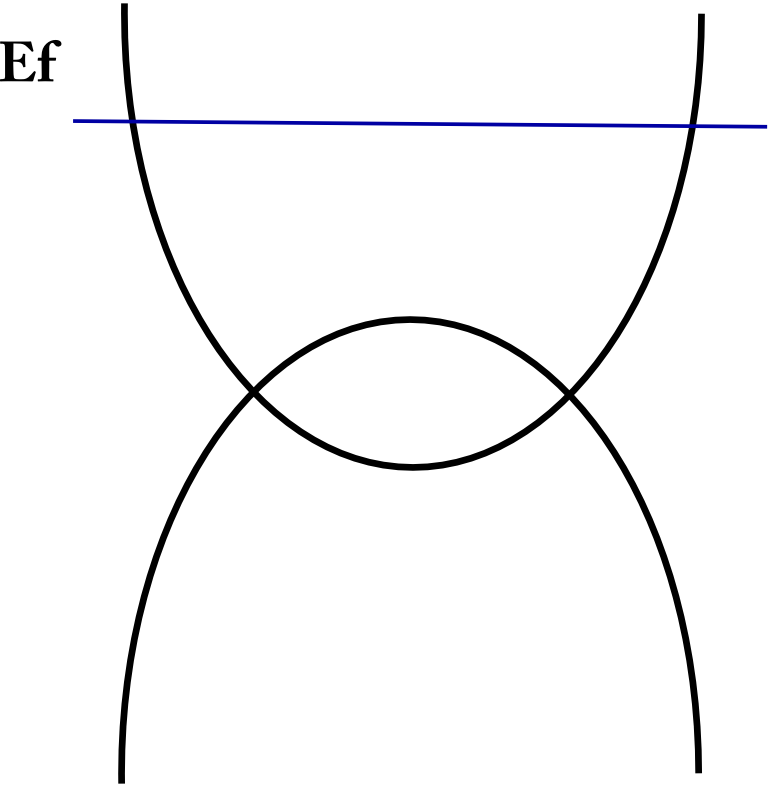
\includegraphics[width=1.75in]{include/metalband.png}\\
\end{wrapfigure}
%Turn off SO Coupling and tune the Fermi energy and now you have a metal,\\
%basis $\{\ket{1\uparrow}, \ket{1\downarrow},\ket{2\uparrow},\ket{2\downarrow} \}$,
$M({\bf k})=M-B_1 k_z ^2 - B_2 (k_x^2 + k_y^2)$
\vspace{1cm}\\
$
H_{Metal}({\bf k})=
$
\vspace{.5cm}\\
$
\left( \begin{array}{cccc}
M({\bf k}) & 0 &0  & 0 \\
0 &M({\bf k})& 0 & 0 \\
0 &0 &-M({\bf k}) & 0 \\
0 & 0 &0 & -M({\bf k}) \\
 \end{array} \right)-E_F 
$\\
\vspace{1cm}
%$M=0.28$ eV,\\ .\\
%$A_1=2.2$ eV\AA, $A_2=4.1$ eV\AA, $B_1=10$ eV\AA$^2$, $B_2=56.6 $ eV\AA$^2$.\\
 %$\mu$ is variable.\\. \\
% H. Zhang et al, Nature Physics 5, 438 (2009)
Then turn on superconductivity ($\Delta$)...

\end{frame}


\begin{frame}{Band Diagram}
%%%%%%%%%%%%%%%%%%%%%%%%%%
\begin{figure}
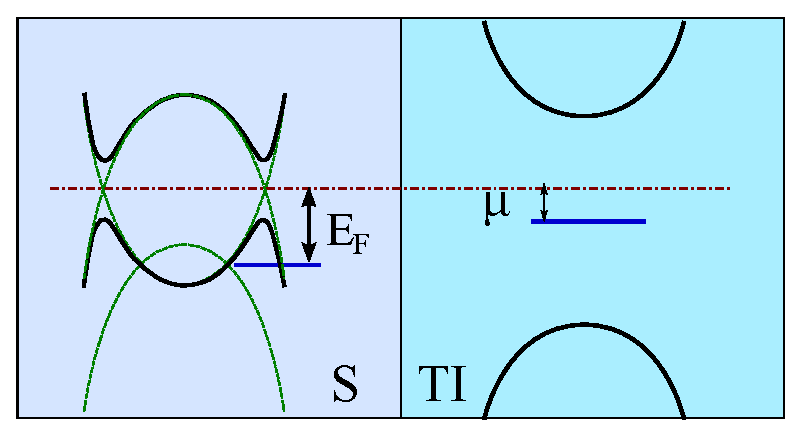
\includegraphics[width=3in]{include/setup.eps}\\
\center
Superconducting gap $<<$ TI Insulating gap
\end{figure}
%%%%%%%%%%%%%%%%%%%%%%%%%%
\end{frame}


\begin{frame}{BdG Hamiltonian}
%The wave function $u$ and $v$ satisfy the following Bogliubov-de Gennes (BdG) equation*,
%\begin{equation*}
%\hat{H}_{B}(\mathbf{k}_\parallel,z) \hat{\phi}_n(\mathbf{k}_\parallel,z)=\epsilon_n(k_\parallel)\hat{\phi}_n (\mathbf{k}_\parallel,z).
%\label{bdgsimp}
%\end{equation*}
8 $\times$ 8 BdG Superconductor-TI Hamiltonian
\begin{equation*}
\hat{H}_{B}=\left( \begin{array}{cccc}
h_0 -\mu  & \mathbf{d} \cdot \boldsymbol{\sigma}&0&0\\ 
 \mathbf{d} \cdot \boldsymbol{\sigma} &-h_0 -\mu &0&-\Delta\, i\sigma_y\\ 
0 &0& \mu -h_0 & \mathbf{d} \cdot \boldsymbol{\sigma}^* \\
0 &\Delta^{\ast} \, i\sigma_y & \mathbf{d} \cdot \boldsymbol{\sigma}^* & \mu+h_0\\ 
 \end{array} \right)
\end{equation*}\\
\begin{equation*}
d_x=A_1(z)k_x,\,\, d_y=A_1(z)k_y,\,\, d_z=A_2(z)(-i\partial_z),
\end{equation*} \\
\begin{equation*}
h_0(\mathbf{k}_\parallel, \partial_z)=M -B_1 \partial_z^2 -B_2 k_\parallel^2
\end{equation*} 
\end{frame}


\begin{frame}{Fourier Expansion}
%%%%%%%%%%%%%%%%%%%%%%%%%%
\begin{figure}
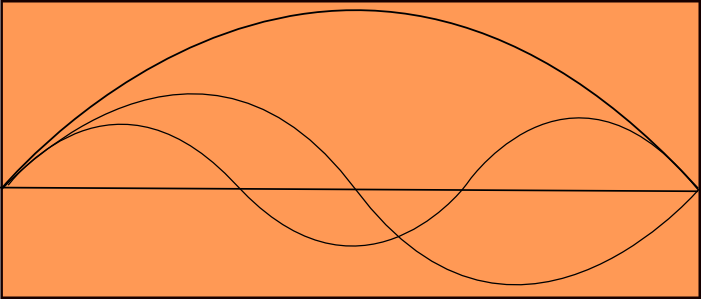
\includegraphics[width=2in]{include/particlebox.png}
\end{figure}
%%%%%%%%%%%%%%%%%%%%%%%%%%
\begin{align*}
u_{n,l\sigma}(z) = \sum_m u_{nm}^{l \sigma}\,\phi_m(z),\quad 
v_{n,l\sigma}(z) = \sum_m v_{nm}^{l \sigma}\, \phi_m(z),\\
\Delta(z) = \sum_m \Delta_{m}\, \phi_m(z) ,\quad 
\phi_m(z)=\sqrt{2/L}\sin(k_m z).
\end{align*}
%The integer $m=1,2,...,N$ labels the quantized $z$ momentum $k_m=m\pi/L$. 
%The cutoff $N$ is chosen as 
%\begin{equation*}
%B_1k^2_N=B_1(N\pi/L)^2=M+E_f+\omega_D. \label{eq-N}
%\end{equation*}
BdG equation becomes an $8N \times 8N$ matrix equation. \\.\\
%Valls et al. (2001)
K. Halterman and O. T. Valls, Phys. Rev. B 65,  014509 (2001)\\
%B. P. Stojkovic and O. T. Valls, Phys. Rev. B 47, 5922 (1993)
\end{frame}


%\begin{frame}{A sample slide}
%\section{the order parameter}

%%%%%%%%%%%%%%%%%%%%%%%%%%
%\begin{figure}
%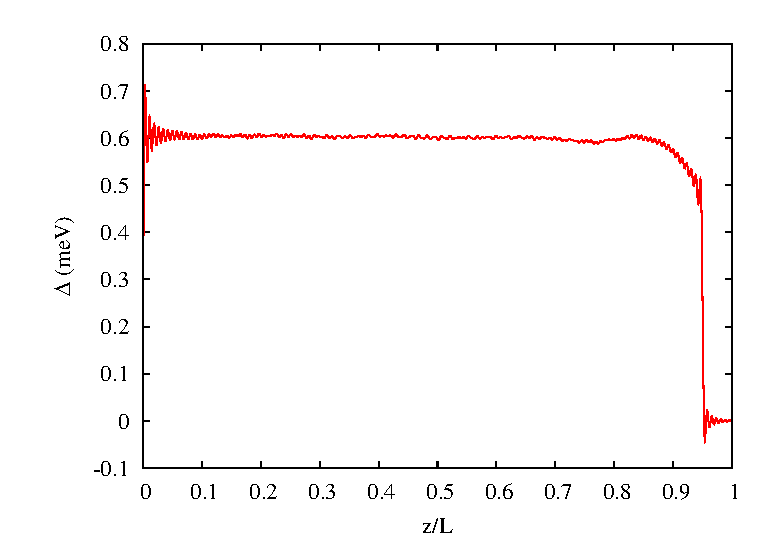
\includegraphics[width=3.4in]{delta-cu.eps}
%\caption{The superconducting order parameter $\Delta(z)$ near an S-TI interface at $
%z=d=0.95L$. The superconductor occupies $0<z<d$, and topological insulator occupies $d<z<L$. 
%$L=300$ nm, $\mu$=0, the bulk gap $\Delta_0=$0.6meV. }\label{delta-cu}
%\end{figure}
%%%%%%%%%%%%%%%%%%%%%%%%%%
%\end{frame}




%\begin{frame}{A sample slide}

%%%%%%%%%%%%%%%%%%%%%%%%%%
%\begin{figure}
%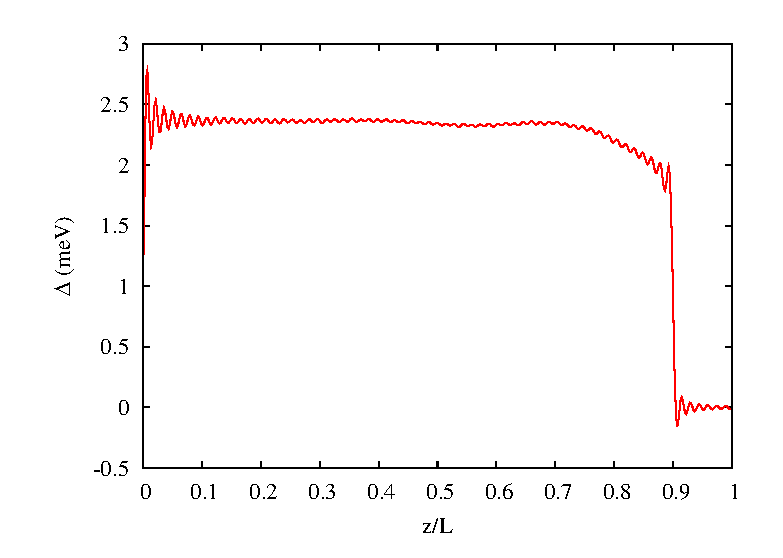
\includegraphics[width=3.4in]{dt.eps}
%\caption{The order parameter $\Delta(z)$ near an S-TI interface at $
%z=d=0.9L$. $L=160$ nm, $\mu$=0, $\Delta_0\sim 2.4$meV.}
%\label{delta-24}
%\end{figure}
%%%%%%%%%%%%%%%%%%%%%%%%%%

%\end{frame}

\begin{frame}{Order Parameter $\Delta$}
%%%%%%%%%%%%%%%%%%%%%%%%%%
\begin{figure}
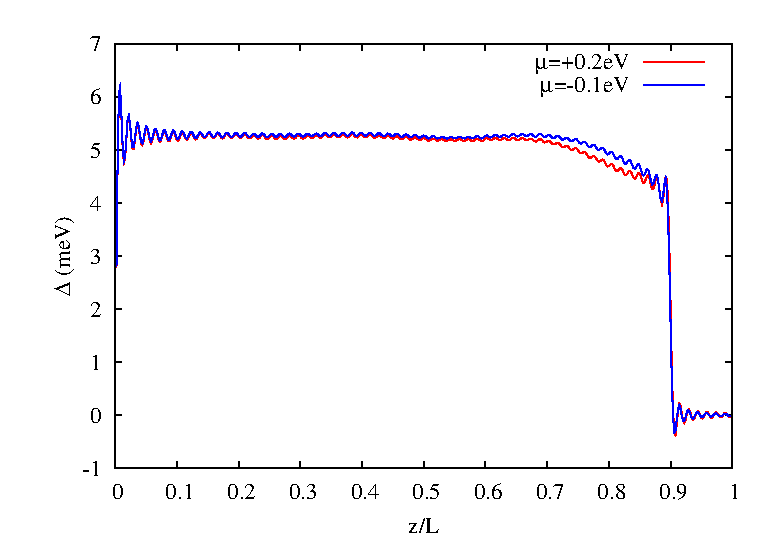
\includegraphics[width=3.4in]{include/dtchemi.eps}\\
 $\mu=-0.1$eV (Blue) and $\mu=0.2$eV (Red)\\ 
$L=160$nm,  $\Delta_0\sim 5.2$meV. 
\end{figure}
%%%%%%%%%%%%%%%%%%%%%%%%%%
\end{frame}




\begin{frame}{Triplet Correlations}
%%%%%%%%%%%%%%%%%%%%%%%%%%
\begin{figure}
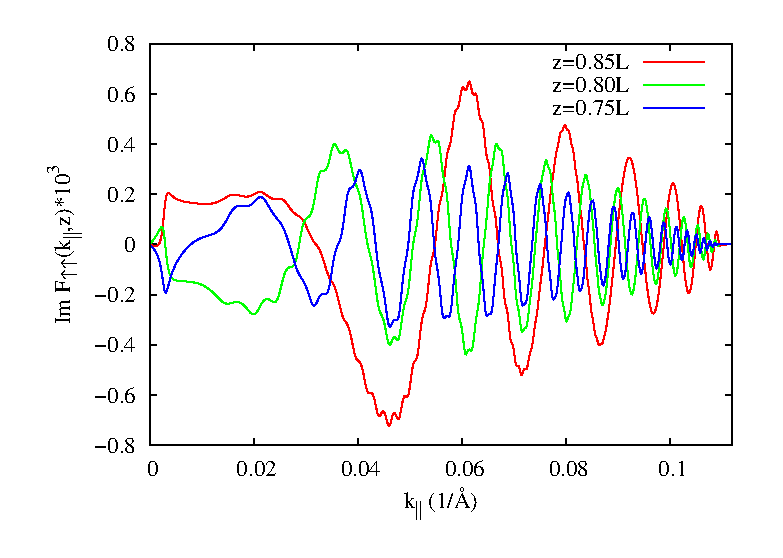
\includegraphics[width=3.4in]{include/pwave.eps}\\
{Im}[$F_{\uparrow\uparrow}(k_\parallel,z)$]:
$d=0.9L$, $\mu=0$, $L=160$nm, $\Delta_0=5.2$meV\\
T. D. Stanescu, et al, Phys. Rev. B 81, 241310 (2010)\\
A. M. Black-Schaffer, Phys. Rev. B 83, 060504 (2011)
\end{figure}
%%%%%%%%%%%%%%%%%%%%%%%%%%
\end{frame}



%\begin{frame}{Triplet Correlations - Low Momentum}
%%%%%%%%%%%%%%%%%%%%%%%%%%
%\begin{figure}
%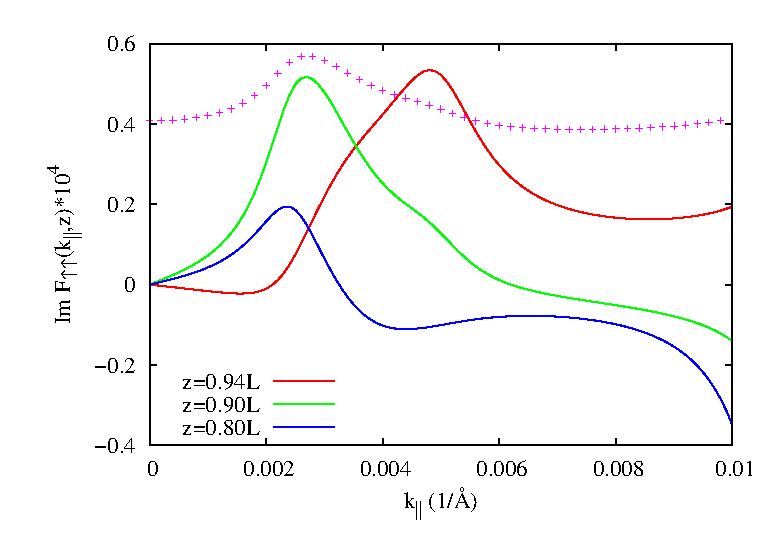
\includegraphics[width=3.4in]{include/pw-cu.eps}\\
%Im[$F_{\uparrow\uparrow}(k_\parallel,z)$]: $\mu=0$, $L=300$nm, $d=0.95L$, %$\Delta_0=0.6$meV\\
%z=\{.94L,.90L,.80L\}\\
%$F_{\uparrow\downarrow}(k_\parallel,z=0.9L)/3$
%\end{figure}
%%%%%%%%%%%%%%%%%%%%%%%%%%
%\end{frame}


\begin{frame}{Fu-Kane Model Verification}
%%%%%%%%%%%%%%%%%%%%%%%%%%
\begin{figure}
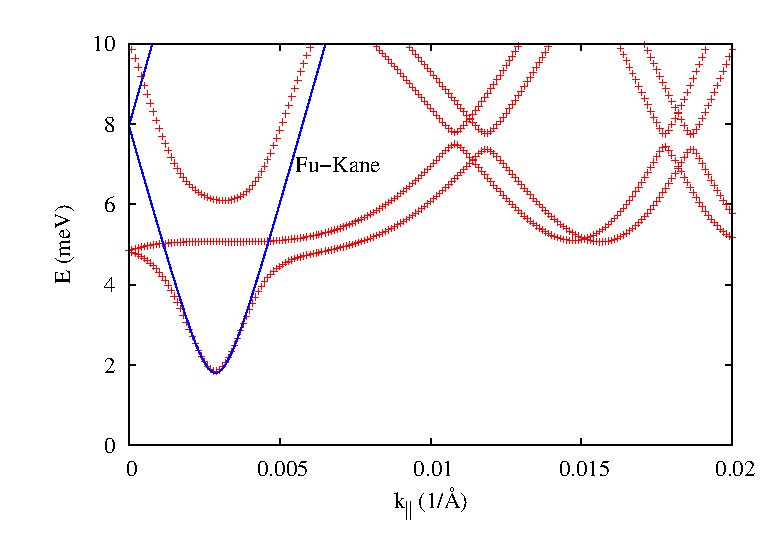
\includegraphics[width=3.4in]{include/levels.eps}\\
$\epsilon_n(k_\parallel)$  
$\mu=0$, $L=160$nm,  $\Delta_0\sim$5.2meV\\
Fu-Kane model fit: $\Delta_s=1.8$meV, $v_s=2.7$eV\AA, and $\mu_s=7.5$meV \\
$E(k)=\sqrt{|\Delta_s|^2+(v_sk \pm\mu_s)^2}$
\end{figure}
%%%%%%%%%%%%%%%%%%%%%%%%%%
\end{frame}



\begin{frame}{Fu-Kane Model Verification - Vary $\mu$}
%%%%%%%%%%%%%%%%%%%%%%%%%%
\begin{figure}
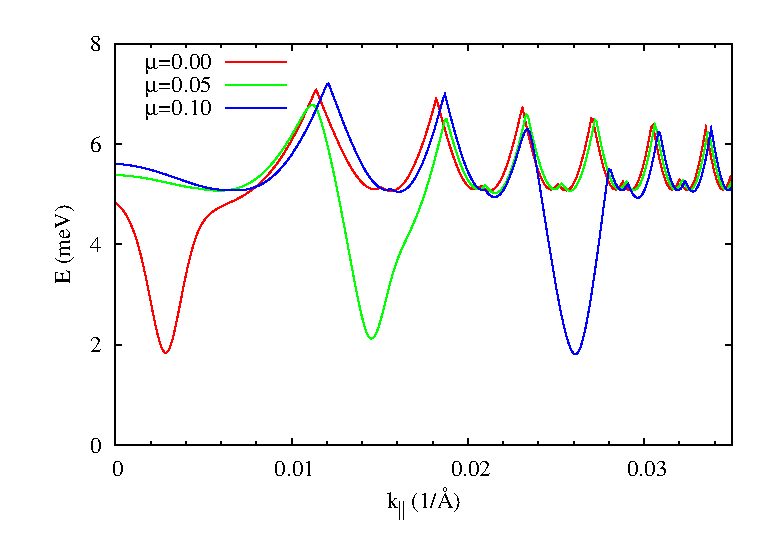
\includegraphics[width=3.4in]{include/disp-mu.eps}\\
$L=160$nm , $\Delta_0\sim$5.2meV \\
$\mu$=\{.00, .05, .10\}eV
\end{figure}
%%%%%%%%%%%%%%%%%%%%%%%%%%
\end{frame}

\begin{frame}{Location of the Fu-Kane Modes}
%%%%%%%%%%%%%%%%%%%%%%%%%%
\begin{figure}
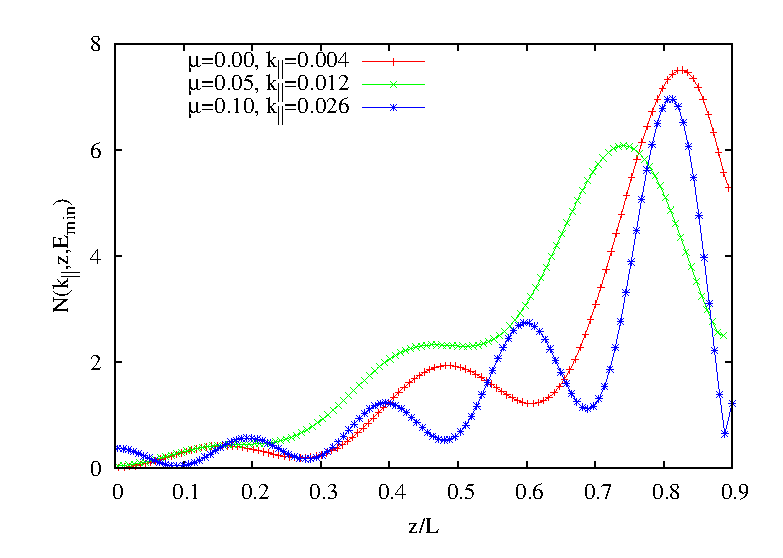
\includegraphics[width=3.4in]{include/spweight.eps}\\
Envelope of $N(k_\parallel,z,\omega)$, $\omega=E_{min}$\\
 $z^\prime=0.9L$, $L$=160nm

\end{figure}
%%%%%%%%%%%%%%%%%%%%%%%%%%
\end{frame}


%\begin{frame}{A sample slide}
%%%%%%%%%%%%%%%%%%%%%%%%%%
%\begin{figure}
%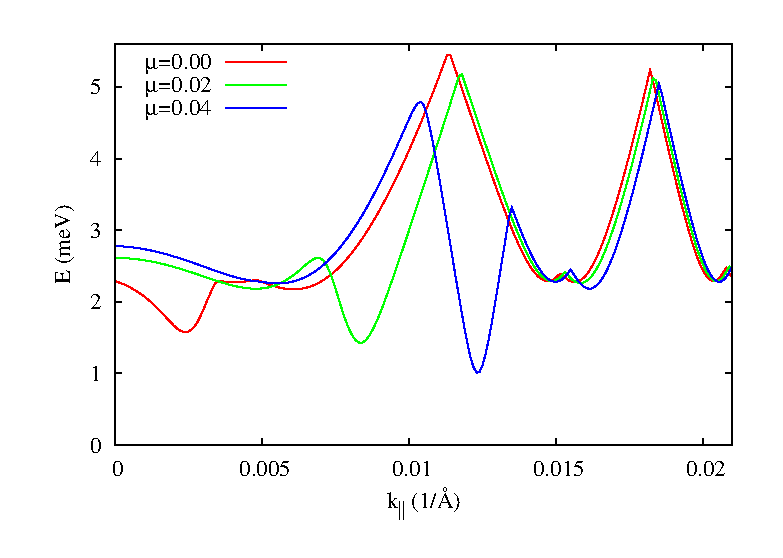
\includegraphics[width=3.4in]{include/spg27.eps}
%\caption{The lowest energy level of an S-TI structure with $L=160$nm, $d=0.9L$, $\Delta_0=2.4$meV. $\mu$ is the chemical potential of the TI and measured in eV.}\label{level-27}
%\end{figure}
%%%%%%%%%%%%%%%%%%%%%%%%%%
%\end{frame}



\begin{frame}{Summary}
\Large
Order parameter is mildly suppressed\\
Induced triplet pairing correlations due to SO coupling\\
Interface modes below the bulk superconducting gap\\
$\quad \rightarrow$ Fu-Kane Model verified, parameters renormalized.\\
\end{frame} 




 %%%%%%%%%%%%%%%%%%%%%%%%%%
 \begin{frame}{}
\Large 
Understanding the bulk effects of the TI are great.\\
How about the surface?
\end{frame}




 %%%%%%%%%%%%%%%%%%%%%%%%%%



 \begin{frame}{Superconducting Josephson Junction Surface}

 %%%%%%%%%%%%%%%%%%%%%%%%%%
\begin{figure}
\center
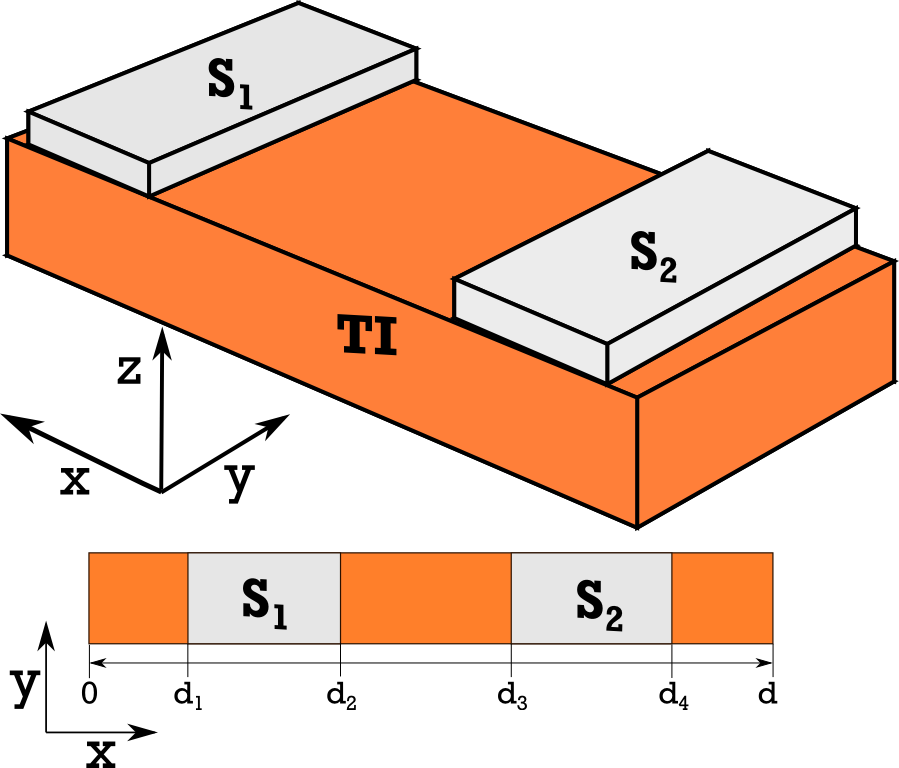
\includegraphics[width=3in]{setup.png}
\label{setup}
\end{figure}
S$_1$ and S$_2$ are the two superconducting leads (Sn, Pb, Al, etc.)
%%%%%%%%%%%%%%%%%%%%%%%%%%
\end{frame} 
 \begin{frame}{Model and Basic Equations}

Surface Dirac-Bogoliubov-de Gennes Hamiltonian,
\begin{eqnarray}
&\mathcal{H}=\left(
\begin{array}{cc}
h_{+}  &  \hat{\Delta} \\
\hat{\Delta}^\dagger  &   h_{-}
\end{array}\label{fkmodel}
\right),&
\end{eqnarray}
where
\begin{eqnarray}
&h_{\pm}= -i\hbar  v_F (\sigma_x\partial_x \pm \sigma_y \partial_y) \mp \mu(x),&\\
&\hat{\Delta}= i\sigma_y  \Delta(x).&
\end{eqnarray}
The basis
\begin{equation}
\psi_n=\left ( { u} _{n\uparrow},  { u}_{n\downarrow},  { v}_{n\uparrow}, { v}_{n\downarrow} \right )^T,
\end{equation} 
which satisfies $ \mathcal{H}\psi_n=\epsilon_n \psi_n, $ represents the BdG particle ($u_\sigma (k_y, x)$), and hole ($v_\sigma (k_y, x)$) 

\end{frame} 


 \begin{frame}{Model and Basic Equations}

Initial order parameter and chemical potential: 
\begin{eqnarray}
\Delta(x)&=&\left\{
\begin{array}{cc}
\Delta_0,&(d_1<x<d_2)\\
\Delta_0 e^{i\phi},& (d_3<x<d_4)\\
0,& \text{elsewhere}\\
\end{array} \right . ,\\
\mu(x)&=&\left\{
\begin{array}{cc}
\mathcal{E}_F,&(d_1<x<d_2) \text{ or } (d_3<x<d_4)\\
\mu,& \text{elsewhere}\\
\end{array} \right .,
\end{eqnarray}

Gap equation
\begin{equation}
\Delta(x)=g(x)\int  d k_y \sum_n^\prime u_{n\uparrow}(k_y, x)v^*_{n\downarrow}(k_y, x)
\end{equation}\label{gap-eq}
\\
$g(x)$: contact pairing potential
\begin{eqnarray}
g(x)=\left\{
\begin{array}{cc}
g_0,&(d_1<x<d_2) \text{ or } (d_3<x<d_4)\\
0,& \text{elsewhere}\\
\end{array} \right .
\end{eqnarray}

\end{frame} 
 \begin{frame}{Model and Basic Equations}


This basis expansion results in a 4N $\times$ 4N matrix Hamiltonian of:
\begin{eqnarray}
&\mathcal{H}=\left(
\begin{array}{cccc}
-\mu_{nm} &  \mathcal{K}^-_{nm} & 0 & \hat{\Delta}_{nm} \\
\mathcal{K}^+_{mn}  & -\mu_{nm}  & -\hat{\Delta}_{nm} & 0 \\
0 & -\hat{\Delta}_{nm}^\ast  & \mu_{nm} &  \mathcal{K}^+_{nm}\\
\hat{\Delta}_{nm}^\ast & 0 &  \mathcal{K}^-_{mn}  & \mu_{nm}
\end{array}\label{fkmodel}
\right),&
\end{eqnarray}
with
\begin{eqnarray}
\mathcal{K}^{\pm}_{nm}&=& -i\hbar  v_F (k_m B_{nm} \pm  k_y \delta_{nm}),\\
B_{nm} &=& \frac{2}{d}\int^d_0  \sin(k_n x) \cos(k_m x) dx\\
\mu_{nm}&=& \frac{2}{d}\int^d_0 \mu(x) \sin(k_n x) \sin(k_m x) dx\\
\hat{\Delta}_{nm}&=&  \frac{2}{d}\int^d_0 \Delta(x) \sin(k_n x) \sin(k_m x) dx
\end{eqnarray}
in the basis of
\begin{equation*}
\psi=  \left ( u_{n\uparrow1}...u_{n\uparrow N}, u_{n\downarrow1}...u_{n\downarrow N}, v_{n\uparrow1}...v_{n\uparrow N}, v_{n\downarrow1}...v_{n\downarrow N}, \right )^T,
\end{equation*} 

Using these techniques, we will solve two different types of SNS Josephson junction structures, one with a phase difference of $\phi=0$ and one with a phase difference of $\phi=\pi$. These two structures offer very different physics.

%%%%%%%%%%%%%%%%%%%%%%%%%%

\clearpage

\end{frame}  


\begin{frame}{Energy Spectrum: Zero Bias Junction}

\begin{figure}[h]
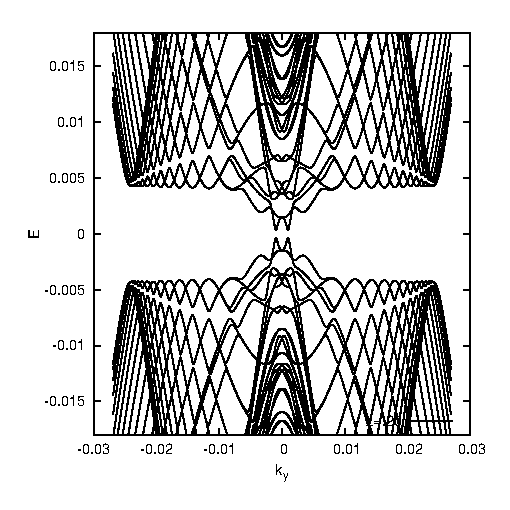
\includegraphics[width=2.9in]{energy_zero}
\caption{Energy spectrum of zero-bias (left) and pi-bias (right) junction. TI chemical potential is set to 5 meV. Energy in units of eV.
}\label{jj-energy}
\end{figure}
\end{frame}  


\begin{frame}{Energy Spectrum: $\pi$ Bias Junction}

\begin{figure}[h]
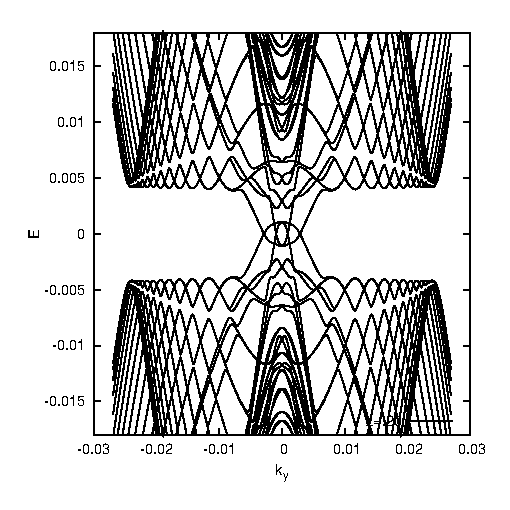
\includegraphics[width=2.9in]{energy_pi}
\caption{Energy spectrum of zero-bias (left) and pi-bias (right) junction. TI chemical potential is set to 5 meV. Energy in units of eV.
}\label{jj-energy}
\end{figure}
\end{frame}  


\begin{frame}{Order Parameter and Singlet Correlation}


\begin{figure}
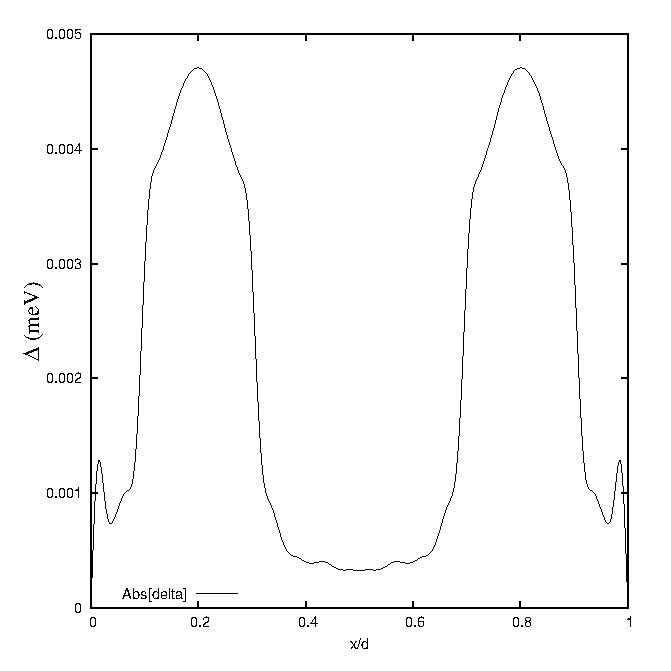
\includegraphics[width=3in]{delta-zero-050}
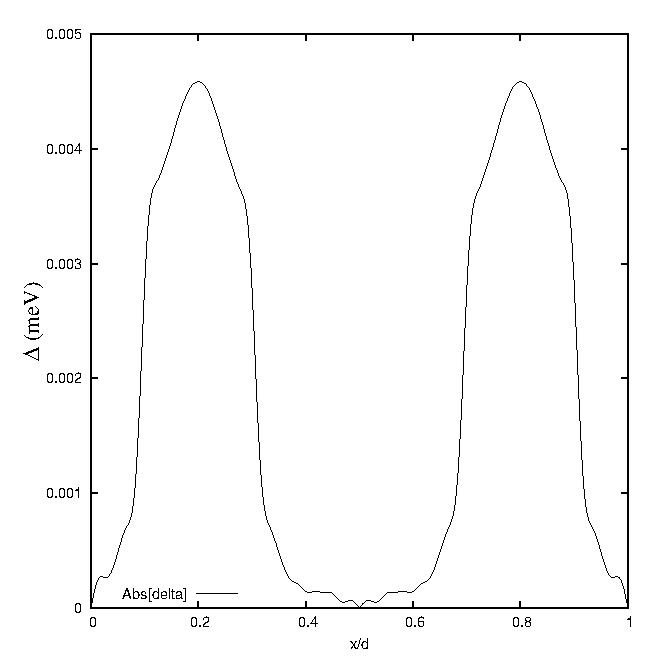
\includegraphics[width=3in]{delta-pi-050}
\caption{The absolute value of the singlet correlation profiles of the zero (left) and $\pi$ (right) junctions. The $\pi$ junction falls to zero at the midpoint. The left side of the midpoint is positive valued while the right side is negative valued. Energy of the order parameter is measured in eV and x/d is the unit-less relative distance along the structure.
}\label{order}
\end{figure}

\clearpage

\end{frame}  

\begin{frame}{Local Density of States: Zero Bias Junction}

\begin{figure}
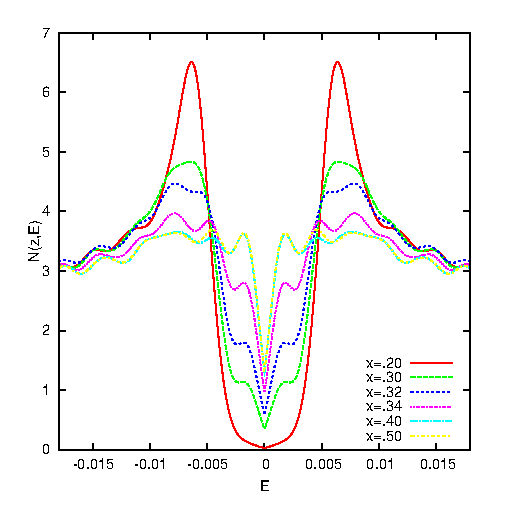
\includegraphics[width=3in]{dos_zero}
\caption{Local density of states at different positions in the heterostructure. Left (right) is the zero ($\pi$) biased junction. Energy in units of eV.
}\label{ldos-jj}
\end{figure}
\end{frame}

\begin{frame}{Local Density of States: $\pi$ Junction}

\begin{figure}
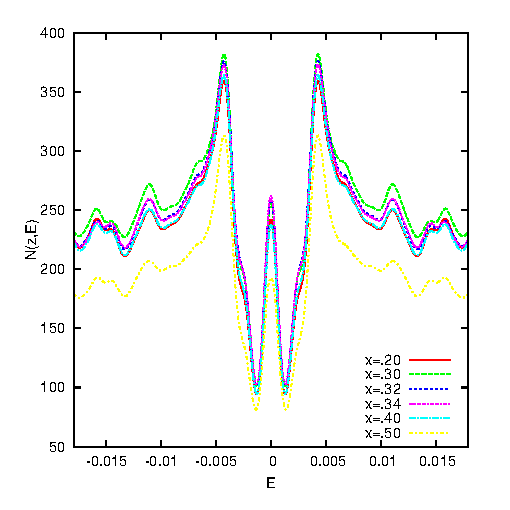
\includegraphics[width=3in]{dos-pi-050}
\caption{Local density of states at different positions in the heterostructure. Left (right) is the zero ($\pi$) biased junction. Energy in units of eV.
}\label{ldos-jj}
\end{figure}

\end{frame}

\begin{frame}{}

\begin{figure}[h]
\center
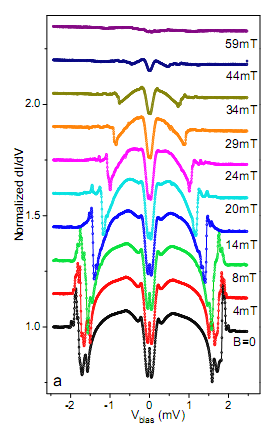
\includegraphics[width=3.2in]{fanyang.png}
\caption{dI/dV curve of experimental results of a S-TI structure from arxiv:1105.0229 (F. Yang et al).
}\label{fanyang}
\end{figure}

\clearpage
\end{frame}  

\begin{frame}{Spectral Function}
\begin{figure}
\center
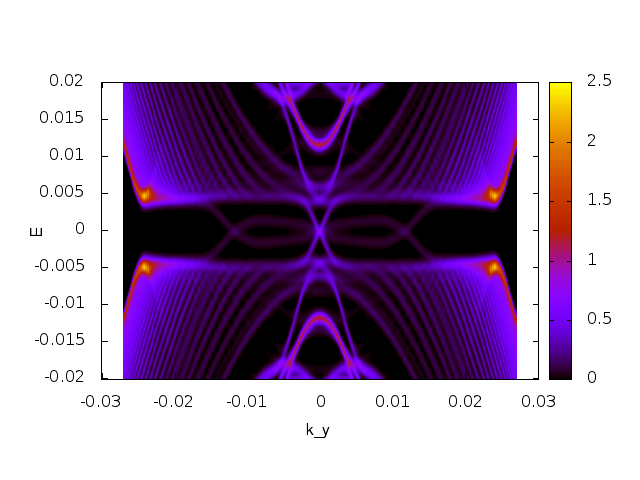
\includegraphics[width=3.8in]{spectral-003.png}
\caption{Local spectral function near the midpoint ($\approx .55$) of the $\pi$ junction heterostructure. Left (right) is the zero ($\pi$) biased junction. Energy in units of eV. k$_y$ in units of \AA$^{-1}$
}\label{spectral-jj}
\end{figure}


\end{frame}  

\begin{frame}{Summary}


\end{frame}  

%%%%%%%%%%%%%%%%%%%%%%%%%%

\begin{frame}{TI-FET: MOSFET with a Topological Insulator}
\begin{figure}[h]
\center
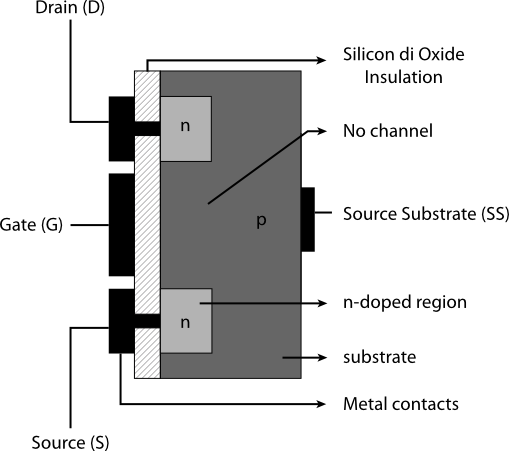
\includegraphics[width=3in]{mosfet.png}
\caption{(left) A proposed heterostructure that exploits the exotic surface states that differ from the bulk in a TI. (right) A typical n-type MOSFET.
}\label{mosfet}
\end{figure}
In this chapter I present ideas proposed by Professor Qialang Li of the Electrical and Computer Engineering department. Professor Li is an expert at electronic device physics and has suggested to utilize a TI in a MOSFET type of structure as a floating gate. In addition it was proposed [need cite] to use a TI as a current channel to provide new characteristics of a transistor.  To give a proper overview of such ideas, I first present a quick introduction on how a MOSFET works, then I show two proposals of structures to be be built. Lastly, I will describe the general outline of how to simulate the physics of these structures to give insight in designing them.

\end{frame}  

\begin{frame}{MOSFET}


\begin{figure}[h]
\center
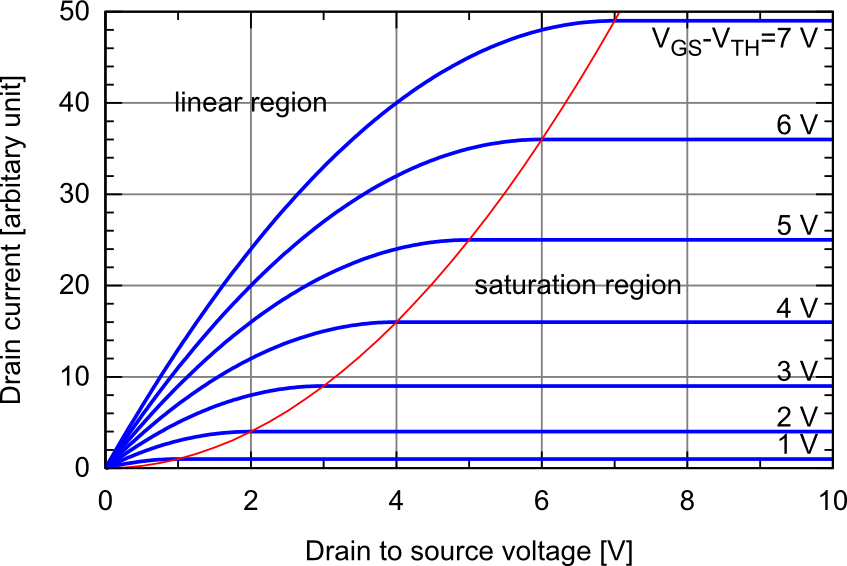
\includegraphics[width=3in]{iv_mosfet.png}
\caption{(left) A proposed heterostructure that exploits the exotic surface states that differ from the bulk in a TI. (right) A typical n-type MOSFET.
}\label{ivmosfet}
\end{figure}

\clearpage
\end{frame}  

\begin{frame}{TI as the Floating Gate}

\begin{figure}[h]
\center
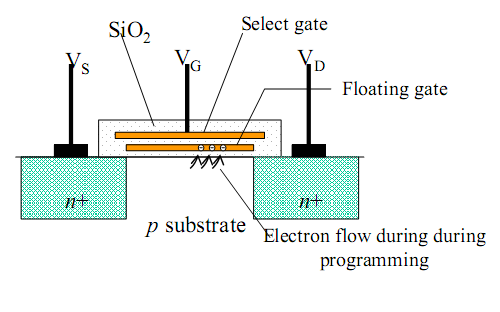
\includegraphics[width=3in]{fgmosfet.png}
\caption{A floating gate MOSFET. The main difference seen here is the additional ``programming gate" above the voltage gate normally seen in a MOSFET.
}\label{fgmosfet}
\end{figure}

\clearpage
\end{frame}  

\begin{frame}{TI as the current channel}

\begin{figure}[h]
\center
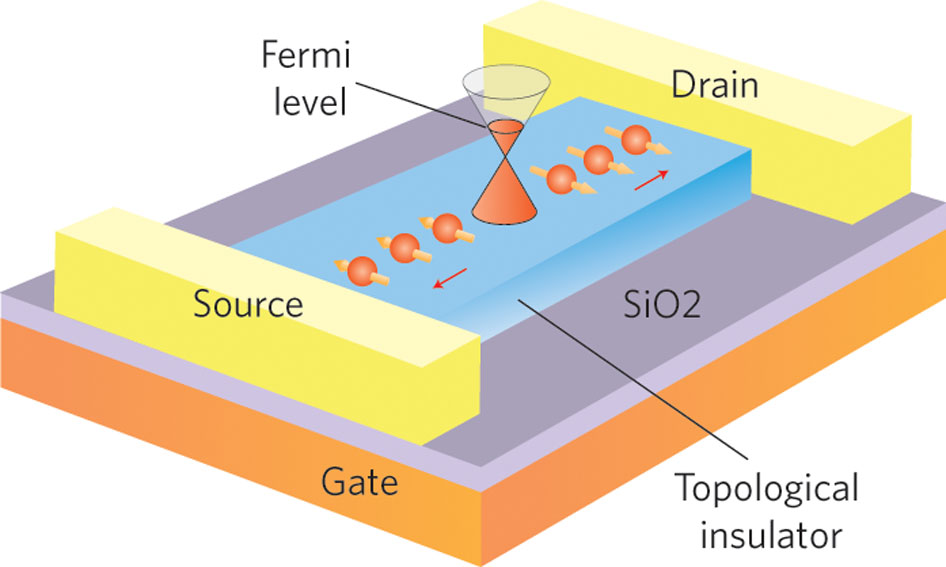
\includegraphics[width=3in]{tifet.jpg}
\caption{(left) A proposed heterostructure that exploits the exotic surface states that differ from the bulk in a TI. (right) A typical n-type MOSFET.
}\label{tifet}
\end{figure}

\end{frame}  

\begin{frame}{}
These calculations are not trivial but should not be extremely computationally intensive. Though the results would be very illuminating, the important factor is the guidance they would give towards performing the experiment in realizing a possible TI-FET structure.

\end{frame}  


\begin{frame}{Summary}
\center \Large Thank you!

\begin{figure}[h]
\center
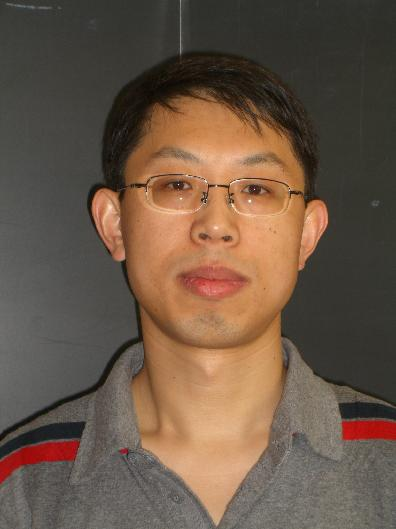
\includegraphics[width=1in]{zhao.jpg}
\includegraphics[width=1.3in]{peja.jpg}
\includegraphics[width=1in]{papa.jpg}
\includegraphics[width=1in]{qli6.jpg}
\end{figure}
\end{frame}  


%\bibliographystyle{aip}
%\bibliography{topological,prox}{}





\begin{frame}{Metal to TI Scattering}
%%%%%%%%%%%%%%%%%%%%%%%%%%
\begin{figure}
\center
\includegraphics[width=1.7in]{f2.pdf}\includegraphics[width=1.7in]{f4.pdf}
\caption{The complex band structure
of topological insulator described by $\hat{H}_{TI}(\v{k})$ 
for $k_y=0$, $k_x=0.02$ (left) and $0.04$ (right). $E$ is measured in eV, and $k$ in $\AA^{-1}$.
Subgap states with complex $k_z$ represent evanescent waves. 
The topology of  real lines \cite{heine63}  changes as $k_x$ is increased.  
}
\end{figure}
%%%%%%%%%%%%%%%%%%%%%%%%%%
\end{frame}
%%%%%%%%%%%%%%%%%




\end{document} 